\documentclass{article}
\iffalse
This file is protected by Copyright. Please refer to the COPYRIGHT file
distributed with this source distribution.

This file is part of OpenCPI <http://www.opencpi.org>

OpenCPI is free software: you can redistribute it and/or modify it under the
terms of the GNU Lesser General Public License as published by the Free Software
Foundation, either version 3 of the License, or (at your option) any later
version.

OpenCPI is distributed in the hope that it will be useful, but WITHOUT ANY
WARRANTY; without even the implied warranty of MERCHANTABILITY or FITNESS FOR A
PARTICULAR PURPOSE. See the GNU Lesser General Public License for more details.

You should have received a copy of the GNU Lesser General Public License along
with this program. If not, see <http://www.gnu.org/licenses/>.
\fi

\author{} % Force author to be blank
%----------------------------------------------------------------------------------------
% Paper size, orientation and margins
%----------------------------------------------------------------------------------------
\usepackage{geometry}
\geometry{
	letterpaper,			% paper type
	portrait,				% text direction
	left=.75in,				% left margin
	top=.75in,				% top margin
	right=.75in,			% right margin
	bottom=.75in			% bottom margin
 }
%----------------------------------------------------------------------------------------
% Header/Footer
%----------------------------------------------------------------------------------------
\usepackage{fancyhdr} \pagestyle{fancy} % required for fancy headers
\usepackage{multirow}
\usepackage{longtable}
\usepackage{footnote}
\renewcommand{\headrulewidth}{0.5pt}
\renewcommand{\footrulewidth}{0.5pt}
\rhead{\small{ANGRYVIPER Team}}
%----------------------------------------------------------------------------------------
% Appendix packages
%----------------------------------------------------------------------------------------
\usepackage[toc,page]{appendix}
%----------------------------------------------------------------------------------------
% Defined Commands & Renamed Commands
%----------------------------------------------------------------------------------------
\renewcommand{\contentsname}{Table of Contents}
\renewcommand{\listfigurename}{List of Figures}
\renewcommand{\listtablename}{List of Tables}
\newcommand{\todo}[1]{\textcolor{red}{TODO: #1}\PackageWarning{TODO:}{#1}} % To do notes
\newcommand{\code}[1]{\texttt{#1}} % For inline code snippet or command line
%----------------------------------------------------------------------------------------
% Various pacakges
%----------------------------------------------------------------------------------------
\usepackage{hyperref} % for linking urls and lists
\usepackage{graphicx} % for including pictures by file
\usepackage{listings} % for coding language styles
\usepackage{rotating} % for sideways table
\usepackage{pifont}   % for sideways table
\usepackage{pdflscape} % for landscape view
%----------------------------------------------------------------------------------------
% Table packages
%----------------------------------------------------------------------------------------
\usepackage{tabularx} % c=center,l=left,r=right,X=fill
\usepackage{float}
\floatstyle{plaintop}
\usepackage[tableposition=top]{caption}
\newcolumntype{P}[1]{>{\centering\arraybackslash}p{#1}}
\newcolumntype{M}[1]{>{\centering\arraybackslash}m{#1}}
%----------------------------------------------------------------------------------------
% Block Diagram / FSM Drawings
%----------------------------------------------------------------------------------------
\usepackage{tikz}
\usetikzlibrary{shapes,arrows,fit,positioning}
\usetikzlibrary{automata} % used for the fsm
\usetikzlibrary{calc} % For duplicating clients
\usepgfmodule{oo} % To define a client box
%----------------------------------------------------------------------------------------
% Colors Used
%----------------------------------------------------------------------------------------
\usepackage{colortbl}
\definecolor{blue}{rgb}{.7,.8,.9}
\definecolor{ceruleanblue}{rgb}{0.16, 0.32, 0.75}
\definecolor{drkgreen}{rgb}{0,0.6,0}
\definecolor{deepmagenta}{rgb}{0.8, 0.0, 0.8}
\definecolor{cyan}{rgb}{0.0,0.6,0.6}
\definecolor{maroon}{rgb}{0.5,0,0}
%----------------------------------------------------------------------------------------
% Update the docTitle and docVersion per document
%----------------------------------------------------------------------------------------
\def\docTitle{Platform Data Sheet}
\def\docVersion{1.3}
%----------------------------------------------------------------------------------------
\date{Version \docVersion} % Force date to be blank and override date with version
\title{\docTitle}
\lhead{\small{\docTitle}}

\def\comp{matchstiq\_z1}
\edef\ecomp{matchstiq_z1}
\def\Comp{matchstiq\_z1 Platform}
\graphicspath{ {figures/} }

\begin{document}

\section*{Summary - \Comp}
\begin{tabular}{|c|M{13.5cm}|}
	\hline
	\rowcolor{blue}
	                  &                                                    \\
	\hline
	Name              & \comp                                              \\
	\hline
	Worker Type       & Platform                                           \\
	\hline
	Version           & v\docVersion \\
	\hline
	Release Date      & February 2018 \\
	\hline
	Component Library & ocpi                                        \\
	\hline
	Workers & \comp.hdl                                        \\
	\hline
\end{tabular}

\section*{Functionality}
\begin{flushleft}
The Matchstiq-Z1 Platform Worker is the interface between the Processing System and the FPGA on the Matchstiq-Z1 Platform. It makes the connections between the AXI buses on the ARM and the OpenCPI Control and Data Planes. Optionally, it can also be used to interface with the SPI, I2C, and UART buses with device workers.
\end{flushleft}

\section*{Worker Implementation Details}
\begin{flushleft}
\begin{figure}[ht]
	\centerline{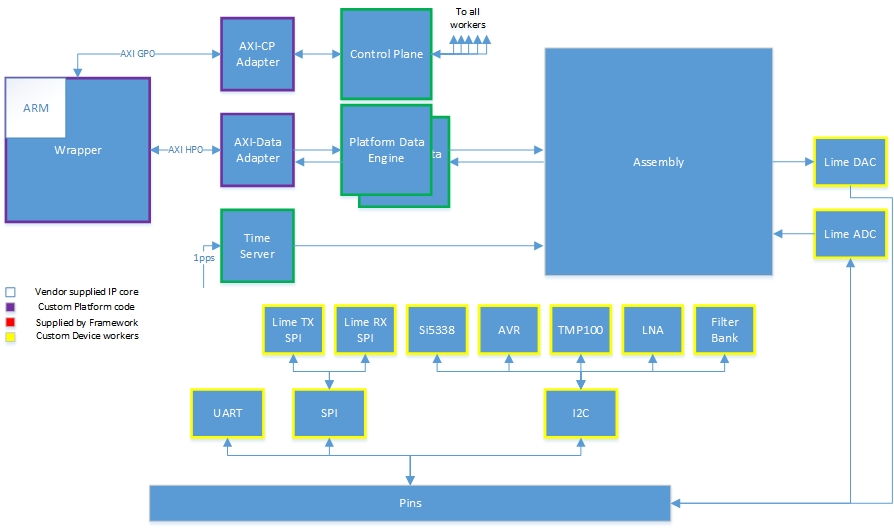
\includegraphics[scale=0.6]{matchstiq_BSP_toplevel}}
	\caption{Top Level Block Diagram}
	\label{fig:top}
\end{figure}

The Matchstiq-Z1 platform has several peripherals connected to the FPGA.  To incorporate these peripherals into the OpenCPI framework, HDL device workers and Software control proxy workers needed to be written.  A overview of these software control proxy workers and HDL Device workers and their interactions can be seen in the diagram below :
\begin{figure}[ht]
	\centerline{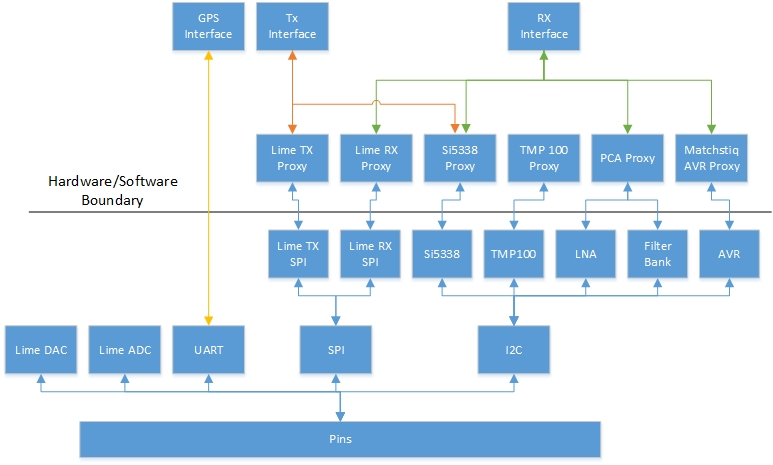
\includegraphics[scale=0.6]{matchstiq_BSP_worker}}
	\caption{Device Worker \& Proxy Diagram}
	\label{fig:wkr}
\end{figure}
\newpage
\subsubsection*{Common Interfaces}
This platform has three different software interfaces, the Rx Interface, Tx interface, and GPS Interface.  The control of the SDR should use these interfaces in order to maintain commonality between different platforms.  More information on each of these interfaces can be found in their respective data sheets.

\begin{figure}[ht]
	\centerline{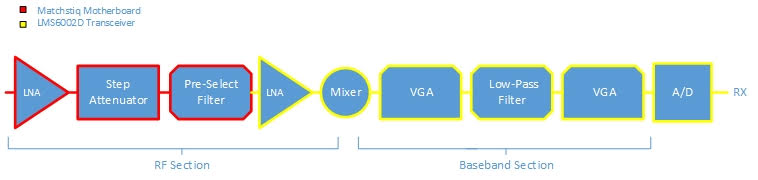
\includegraphics[scale=0.6]{matchstiq_FE_RX_HW}}
	\caption{Receiver Hardware Diagram}
	\label{fig:rx}
\end{figure}
\begin{figure}[ht]
	\centerline{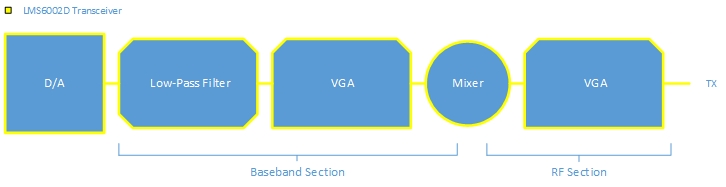
\includegraphics[scale=0.6]{matchstiq_FE_TX_HW}}
	\caption{Transmitter Hardware Diagram}
	\label{fig:tx}
\end{figure}

\end{flushleft}
\pagebreak

\section*{Theory}
Because there are no data processing algorithms implemented in this worker, no corresponding data processing theory is relevant herein.

\section*{Block Diagrams}
\subsection*{Top level}
\makeatletter
\newcommand{\gettikzxy}[3]{%
  \tikz@scan@one@point\pgfutil@firstofone#1\relax
  \edef#2{\the\pgf@x}%
  \edef#3{\the\pgf@y}%
}
\makeatother
\pgfooclass{clientbox}{ % This is the class clientbox
    \method clientbox() { % The clientbox
    }
    \method apply(#1,#2,#3,#4) { % Causes the clientbox to be shown at coordinate (#1,#2) and named #3
        \node[rectangle,draw=white,fill=white] at (#1,#2) (#3) {#4};
    }
}
\pgfoonew \myclient=new clientbox()
\begin{center}
  \begin{tikzpicture}[% List of styles applied to all, to override specify on a case-by-case
      every node/.style={
        align=center,      % use this so that the "\\" for line break works
        minimum size=2cm,  % creates space above and below text in rectangle
        minimum width=4cm
      },
      every edge/.style={draw,thick}
    ]
    \node[rectangle,ultra thick,draw=black,fill=blue](R2){\Comp};
    \node[rectangle,draw=white,fill=white,minimum size=1.0cm](R5)[below= of R2]{timebase};
    \node[rectangle,draw=white,fill=white](placeholder)[above= of R2]{};
    \path[->]
    (R2)edge []  node [] {} (R5)
    (R5)edge []  node [] {} (R2)
    ;
    \gettikzxy{(placeholder)}{\rx}{\ry}
    \myclient.apply(\rx - 50,\ry,C1,\\ metadata);
    \path[<->]($(R2.north) + (-50 pt,0)$) edge [] node [] {} (C1);
    \myclient.apply(-\rx + 50,\ry,C1, ``zynq'' \\ scalable data plane );
    \path[<->]($(R2.north) + (50 pt,0)$) edge [] node [] {} (C1);
    \myclient.apply(-\rx,\ry+50,C1, \\ cpmaster);
    \path[<->]($(R2.north) + (0 pt,0)$) edge [] node [] {} (C1);

  \end{tikzpicture}
\end{center}

\subsection*{State Machines}
Various state machines exist in the zynq, axi, and sdp primitive libraries. See primitive library source code for details. The explicit source code files included in the aforementioned primitives are enumerated in the following section.

\newpage
\section*{Source Dependencies}
\begin{itemize}
	\item
ocpiassets/hdl/platforms/matchstiq\_z1/matchstiq\_z1.vhd
	\item
opencpi/hdl/primitives/zynq/zynq\_pkg.vhd
	\item
opencpi/hdl/primitives/zynq/zynq\_ps.vhd
	\item
opencpi/hdl/primitives/axi/axi\_pkg.vhd
	\item
opencpi/hdl/primitives/axi/axi2cp.vhd
	\item
opencpi/hdl/primitives/sdp/sdp2axi\_rd.vhd
	\item
opencpi/hdl/primitives/sdp/sdp2axi.vhd
	\item
opencpi/hdl/primitives/sdp/sdp2axi\_wd.vhd
	\item
opencpi/hdl/primitives/sdp/sdp\_axi\_pkg.vhd
	\item
opencpi/hdl/primitives/sdp/sdp\_pkg.vhd
	\item
opencpi/hdl/primitives/sdp/sdp\_body.vhd
\end{itemize}

\begin{landscape}
	\section*{Component Spec Properties}
	\begin{scriptsize}
		\begin{tabular}{|p{3cm}|p{1.5cm}|c|c|c|p{1.5cm}|p{1cm}|p{6cm}|}
			\hline
			\rowcolor{blue}
			Name               & Type   & SequenceLength & ArrayDimensions & Accessibility      & Valid Range & Default & Usage                                                                         \\
			\hline
			\verb+platform+    & String & 31             & -               & Parameter & Standard & - & Name of this platform                                                     \\
			\hline
			\verb+sdp_width+   & UChar  & -              & -               & Parameter & Standard & 1 & Width of data plane in DWORDS                                             \\
			\hline
			\verb+UUID+        & ULong  & -              & 16              & Readable           & Standard    & -       & UUID of this platform                                                         \\
			\hline
			\verb+oldtime+     & ULongLong & -           & -               & Padding            & Standard    & -       & N/A                                                                           \\
			\hline
			\verb+romAddr+     & UShort & -              & -               & Writable           & Standard    & -       &                                                                               \\
			\hline
			\verb+romData+     & ULong  & -              & -               & Volatile           & Standard    & -       &                                                                               \\
			\hline
			\verb+nSwitches+   & ULong  & -              & -               & Readable           & Standard    & -       & Number of switches                                                            \\
			\hline
			\verb+nLEDs+       & ULong  & -              & -               & Readable           & Standard    & -       & Number of LEDs                                                                 \\
			\hline
			\verb+memories_length+ & ULong & -           & -               & Readable           & Standard    & -       &                                                                               \\
			\hline
			\verb+memories+    & ULong  & -              & 4               & Readable           & Standard    & -       & The memory regions that may be used by \\
  	                     &        &                &                 &                    &             &         & various other elements, which          \\
  	                     &        &                &                 &                    &             &         & inidicates aliasing etc.               \\
                         &        &                &                 &                    &             &         & The values describing each region are: \\
                         &        &                &                 &                    &             &         & Bit 31:28 - External bus/BAR connected \\
                         &        &                &                 &                    &             &         &             to this memory (0 is none) \\
                         &        &                &                 &                    &             &         & Bit 27:14 - Offset in bus/BAR of this  \\
                         &        &                &                 &                    &             &         &             memory (4KB units)         \\
                         &        &                &                 &                    &             &         & Bit  13:0 - Size of this memory (4KB units) \\
                         &        &                &                 &                    &             &         &             units) \\
			\hline
			\verb+dna+         & ULongLong & -           & -               & Readable           & Standard    & -       & DNA (unique chip serial number) of this platform \\
			\hline
			\verb+switches+    & ULong  & -              & -               & Volatile           & Standard    & -       & Current value of any switches in the platform                                 \\
			\hline
			\verb+LEDS+        & ULong  & -              & -               & Writable, Readable & Standard    & -       & Setting of LEDs in the platform, with readback                                \\
			\hline
			\verb+nSlots+      & ULong  & -              & -               & Parameter & Standard & 0 & Number of slots available for cards, which indicates the usable length of the slotCardIsPresent array property. \\
			\hline
			\verb+slotNames+   & String & 32             & -               & Parameter & Standard & "" & A string which is intended to include comma-separated names of the slots available for cards. The inter-comma position of each name corresponds to the same index of the slotCardIsPresent array property. \\
			\hline
			\verb+slotCardIsPresent+ & Bool & -          & 64              & Volatile           & Standard    & -       & An array of booleans, where each index contains an indication whether a card is physically present in the given index's slot. For a description of a given index's slot, see the corresponding comma-separated string contents in the slotName property. Note that only the first min(nSlots,64) of the 64 indices contain pertinent information. \\
			\hline

		\end{tabular}
	\end{scriptsize}
	\section*{Worker Properties}
	\begin{scriptsize}
		\begin{tabular}{|p{1.5cm}|p{2.5cm}|p{1.5cm}|c|c|c|p{2cm}|p{2cm}|p{3cm}|}
			\hline
			\rowcolor{blue}
			Property Type & Name                  & Data Type  & SequenceLength & ArrayDimensions & Accessibility       & Valid Range & Default & Usage                        \\
			\hline
			SpecProperty & \verb+platform+       & String & 31            & -               & Parameter           & Standard    & matchstiq\_z1 & Name of this platform  \\
			\hline
			Property     & \verb+useGP1+         & Bool   & -             & -               & Parameter           & Standard    & false   &                              \\
			\hline
			Property     & \verb+axi_error+      & Bool   & -             & 4               & Volatile            & Standard    & -       &                              \\
			\hline
			Property     & \verb+sdpDropCount+   & UChar  & -             & -               & Volatile            & Standard    & -       &                              \\
			\hline
			Property     & \verb+debug_state+    & ULongLong & -          & 4               & Volatile            & Standard    & -       &                              \\
			\hline
			Property     & \verb+debug_state1+   & ULongLong & -          & 4               & Volatile            & Standard    & -       &                              \\
			\hline
			Property     & \verb+debug_state2+   & ULongLong & -          & 4               & Volatile            & Standard    & -       &                              \\
			\hline
		\end{tabular}
	\end{scriptsize}

	\section*{Component Ports}
	No ports are implemented for the given component specification.

	\section*{Worker Interfaces}
	\begin{scriptsize}
		\begin{tabular}{|M{2cm}|M{2cm}|M{1.5cm}|M{1.5cm}|M{14.5cm}|}
			\hline
			\rowcolor{blue}
			Type       & Name & Master & Count & Usage                  \\
			\hline
			metadata   & -    & true   & -     & Access to container metadata via the platform worker. All platform workers must provide this port. \\
			\hline
			timebase   & -    & true   & -     & Providing a timebase for the time service. All platform workers must provide this port. \\
			\hline
			cpmaster   & -    & true   & -     & This platform worker provides a control plane. \\
			\hline
			sdp        & zynq & true   & 4     & Scalable data plane. \\
			\hline
		\end{tabular}
	\end{scriptsize}

\end{landscape}
\pagebreak
	\section*{Worker Devices}
	The following is a table which enumerates which device workers are allowed in platform configurations and in assembly containers. The parameter values specified restrict allowed implementations. Note that the worker signals listed are only those who are unconnected on the platform or whose platform signal name differ from the worker signal name. Note that device workers allowed by cards are not included in this list.\\
			\begin{tabular}{|M{3cm}|M{3.5cm}|M{3cm}|M{3cm}|M{3cm}|}
			\hline
			\rowcolor{blue}
			Name                       & Property Name    & Property Value              & Worker Signal & Platform Signal         \\
			\hline
			time\_server               & frequency        & 100*10\textsuperscript{6}   &               &                         \\
			\hline
      \multirow{6}{*}{lime\_adc} &USE\_CLK\_OUT\_p  & 1                           &               &                         \\
                                 &USE\_CLK\_IN\_p   & 0                           &               &                         \\
                                 &USE\_CTL\_CLK\_p  & 0                           &               &                         \\
                                 &DRIVE\_CLK\_p     & 0                           &               &                         \\
                                 &                  &                             & RX\_CLK       & -                       \\
                                 &                  &                             & RX\_CLK\_IN   & -                       \\
			\hline
      \multirow{3}{*}{lime\_dac} &USE\_CLK\_IN\_p   & 1                           &               &                         \\
                                 &USE\_CTL\_CLK\_p  & 0                           &               &                         \\
                                 &                  &                             & TX\_CLK\_IN   & lime\_adc\_rx\_clk\_out \\
			\hline
			lime\_spi                  &                  &                             &               &                         \\
			\hline
			lime\_rx                   &                  &                             & rxen          & -                       \\
			\hline
			lime\_tx                   &                  &                             & txen          & -                       \\
			\hline
			gps\_uart                  &                  &                             &               &                         \\
			\hline
      \multirow{2}{*}{si5338}    &CLKIN\_PRESENT\_p & 1                           &               &                         \\
                                 &CLKIN\_FREQ\_p    & 30.72*10\textsuperscript{6} &               &                         \\
			\hline
			matchstiq\_z1\_avr         &                  &                             &               &                         \\
			\hline
			pca9534                    &                  &                             &               &                         \\
			\hline
			pca9535                    &                  &                             &               &                         \\
			\hline
			tmp100                     &                  &                             &               &                         \\
			\hline
			matchstiq\_z1\_i2c         &                  &                             &               &                         \\
			\hline
		\end{tabular}

\section*{Signals}
Note that this signal table does not include signals that may be provided by slots. \\
\begin{tabular}{|c|c|c|c|p{8cm}|}
	\hline
	\rowcolor{blue}
	Name           & Type   & Differential & Width & Description                                          \\
	\hline
	SI5338\_CLK0A  & Input  & false        & 1     & Differential clock input from Si5338 Clock Generator \\
	\hline
	SI5338\_CLK0B  & Input  & false        & 1     & Differential clock input from Si5338 Clock Generator \\
	\hline
	LIME\_RX\_CLK  & Output & false        & 1     & Single ended clock output to Lime RX\_CLK pin        \\
	\hline
	clocktest      & Output & false        & 1     & Copy of LIME\_RX\_CLK. Pin 3 of rear debug connector \\
	\hline
	GPS\_1PPS\_IN  & Input  & false        & 1     & 1 PPS output from GPS module                         \\
	\hline
	GPS\_FIX\_IND  & Input  & false        & 1     & Fix indication output from GPS module                \\
	\hline
	EXT\_1PPS\_OUT & Output & false        & 1     & 1 PPS output from FPGA                               \\
	\hline
	ATLAS\_LEDS    & Output & false        & 3     & LEDs on ATLAS module                                 \\
	\hline
\end{tabular}
\pagebreak
\section*{Slots}
No slots exist in this platform.
\section*{Platform Configurations}
	\begin{tabular}{|c|c|c|c|}
		\hline
		\rowcolor{blue}
		Name & Platform Configuration Workers & Card & Slot \\
		\hline
		\multirow{2}{*}{base} &\comp & - & - \\ &time\_server & - & - \\
		\hline
		\multirow{9}{*}{matchstiq\_z1\_rx\_tx} &\comp & - & - \\ &time\_server & - & - \\ &si5338 & - & - \\ &tmp100 & - & - \\ &pca9535 & - & - \\ &matchstiq\_z1\_avr & - & - \\ &lime\_rx & - & - \\ &lime\_tx & - & - \\ &gps\_uart & - & - \\
		\hline
		\multirow{8}{*}{matchstiq\_z1\_tx} &\comp & - & - \\ &time\_server & - & - \\ &si5338 & - & - \\ &tmp100 & - & - \\ &pca9535 & - & - \\ &matchstiq\_z1\_avr & - & - \\ &lime\_rx & - & - \\ &gps\_uart & - & - \\
		\hline
		\multirow{7}{*}{matchstiq\_z1\_rx} &\comp & - & - \\ &time\_server & - & - \\ &si5338 & - & - \\ &tmp100 & - & - \\ &matchstiq\_z1\_avr & - & - \\ &lime\_tx & - & - \\ &gps\_uart & - & - \\
		\hline
	\end{tabular}

\section*{Control Timing and Signals}
\subsection*{Control Domain}
All control clocking in the Matchstiq-Z1 platform originates from the PS7 processing clock 1 (FCLK1), which is set to 100 MHz.

\subsection*{Sampling Domain}
The sampling clock domain originates from  the CLK0 output of a SI5338 clock generator, which is connected directly to the Zynq FPGA. The platform worker converts this clock from differential to single ended and outputs this converted clock to the Lime transceiver.\par\medskip
\noindent This clock returns as an input to the Zynq FPGA aligned with the ADC data. This clock is connected as an input signal to the lime\_adc and lime\_dac device workers. See the diagram below for more details.\par\medskip
\begin{figure}[ht]
	\centerline{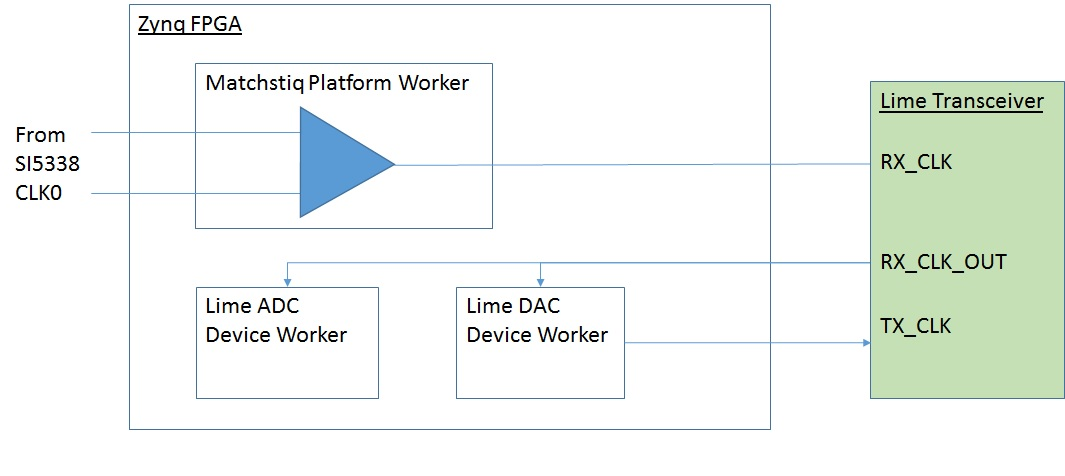
\includegraphics[scale=0.5]{matchstiq_sample_clock_diagram}}
	\caption{Clock Diagram}
	\label{fig:clk}
\end{figure}
\noindent Note that the Lime DAC device worker can also be configured at build time to use an independent clock, the control clock or the sample clock. The default configuration presented here uses the sample clock.
\newpage

\section*{Performance and Resource Utilization}
In the following Platform Worker Utilization tables, the Worker Build Configuration ``0'' refers to the Platform Worker itself. Named configurations refer to platform configurations (\textit{e.g.} they may include other device workers along with the Platform Worker).\\\\

\input{../../\ecomp/utilization.inc}
\section*{Test and Verification}
\begin{flushleft}
 To be detailed in a future release.
\end{flushleft}
\section*{Example Design}
This example design provides the infrastructure necessary to stream samples to/from the DAC/ADC interfaces to file.\par\medskip

\noindent To build the example design, enter the example\_design directory and type `make'.\par\medskip

\noindent To run the example design, NFS mount the example\_design directory on the Matchstiq-Z1 and run the executable in the linux-x13\_3-arm directory.\par\bigskip

\end{document}
